\chapter{السطوح والامتزاز والحفز غير المتجانس}\label{ch:b3:surfaces-catalysis}

تحت السيارة، داخل علبة من الفولاذ، يقبع قرص خزفي على شكل خلية نحل، آلاف
قنواته مكسوّة بأكسيد مسامي يحمل بضعة غرامات من البلاتين 
والبلاديوم والروديوم. وفي جزء من الثانية، تفقد غازات العادم المارة
عبره معظم ما فيها من أحادي أكسيد الكربون والهيدروكربونات غير المحترقة 
وأكاسيد النيتروجين. ولا يحدث شيء في الطور الغازي: فكل تفاعل من هذه التفاعلات يجري
على سطح الجسيمات الفلزية، التي يبلغ قطرها بضعة نانومترات. ومعظم
الصناعة الكيميائية يعمل على هذا النحو، من أمونيا الأسمدة إلى
تكسير البترول. ويصف هذا الفصل كيف تلتصق الجزيئات
بالسطوح، وأي قدر من السطح تغطيه، وكيف تجري التفاعلات السطحية، 
وكيف يُصنع الحفاز الصلب ويُقاس ويُفحص.

\begin{recall}
عرّف مجلد السنة الأولى الحفازات والفرق بين الحفز المتجانس 
والحفز غير المتجانس، ووصف الرصّ المكعب الممركز الأوجه في
الفلزات. وعرّف مجلد السنة الثانية التحويل والانتقائية 
وتردد الدوران لحفاز، ومبدأ لوشاتلييه.
وقدّم \cref{ch:b3:x-ray-diffraction} \omterm{def:b3:x-ray-diffraction:miller}{قرائن ميلر}،
و\cref{ch:b3:rate-theories} \omterm{thm:b3:rate-theories:eyring}{معادلة أيرنغ}
و\cref{ch:b3:partition-functions} إحصاء التوزيعات.
\end{recall}

\begin{omfigure}
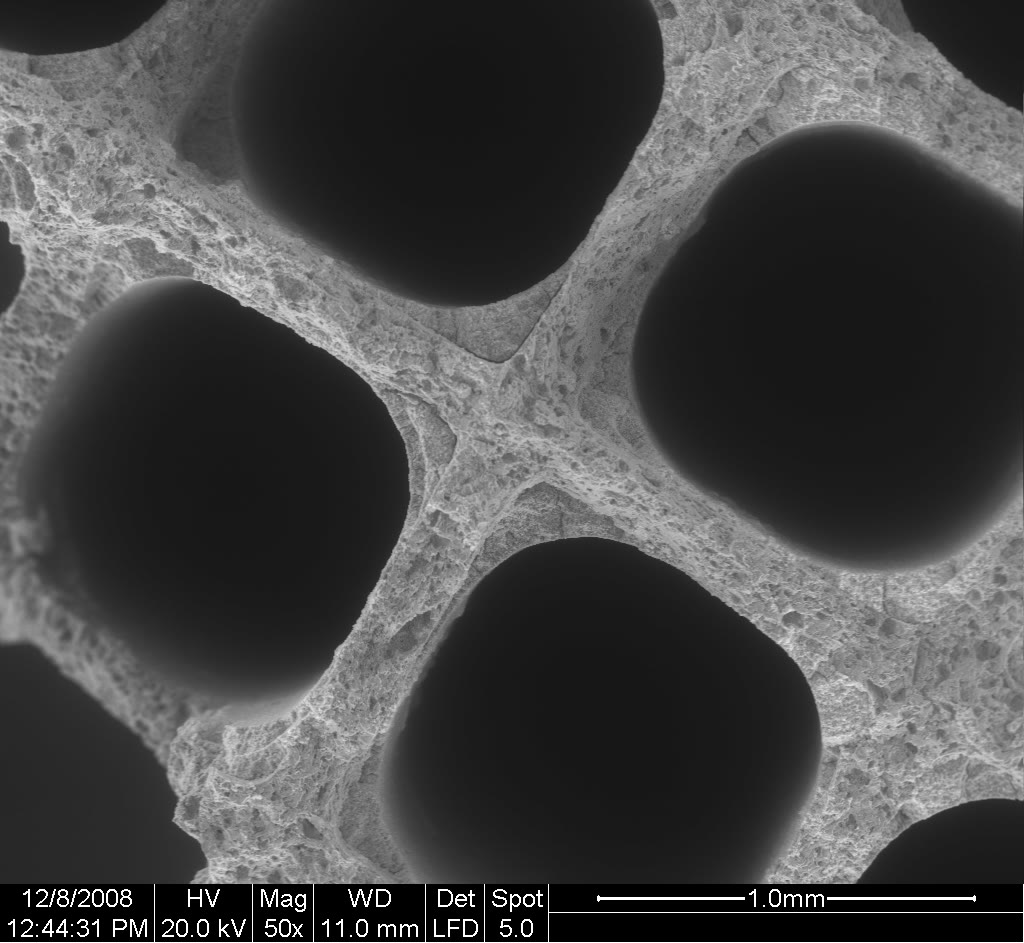
\includegraphics[width=0.48\linewidth]{images/book4/converter-sem.jpg}

{\small القرص الخزفي ذو خلايا النحل في محوّل حفزي كما يُرى بالمجهر الإلكتروني
الماسح (مقياس الرسم \qty{1.0}{mm}): قنوات مربعة تفصلها جدران رقيقة
مسامية، تحمل طبقة الأكسيد الحاملة وجسيماتها الفلزية.}
\end{omfigure}

\section{الامتزاز}

\begin{definition}[الامتزاز]\label{def:b3:surfaces-catalysis:adsorption}
\emph{الامتزاز}\index{امتزاز} هو تراكم جزيئات غاز أو
مذاب على سطح صلب أو سائل. والجزيء الذي يُمتز هو
\emph{المادة الممتزة}\index{مادة ممتزة}، والصلب هو \emph{المادة المازّة}\index{مادة مازة}؛
والعملية العكسية هي \emph{الانتزاز}\index{انتزاز}.
\end{definition}

\begin{definition}[الامتزاز الفيزيائي، الامتزاز الكيميائي]\label{def:b3:surfaces-catalysis:physi-chemi}
\emph{الامتزاز الفيزيائي}\index{امتزاز فيزيائي} \omterm{def:b3:surfaces-catalysis:adsorption}{امتزاز} بقوى فان دير فالس،
بأنتالبيات \omterm{def:b3:surfaces-catalysis:adsorption}{امتزاز} لا تتجاوز بضع عشرات من الكيلوجول لكل مول،
مماثلة لأنتالبيات التكاثف، ودون أي تغير في الجزيء. أما
\emph{الامتزاز الكيميائي}\index{امتزاز كيميائي} فيكوّن روابط كيميائية مع السطح،
بأنتالبيات من نحو 40 إلى عدة مئات من الكيلوجول لكل مول؛ وقد
يكسر الجزيء (\omterm{def:b3:surfaces-catalysis:adsorption}{امتزاز} كيميائي تفككي) ويتوقف عند طبقة واحدة.
\end{definition}

\begin{omfigure}
\begin{tikzpicture}[font=\small, >=Stealth, x=1cm, y=1cm]
  \draw[->] (0,-2.6) -- (0,1.8) node[anchor=south] {\foreignlanguage{arabic}{الطاقة}};
  \draw[->] (0,0) -- (8.0,0) node[anchor=south east] {\foreignlanguage{arabic}{البعد عن السطح}};
  \draw[omDef, thick] plot[smooth, tension=0.7] coordinates {(1.6,1.6) (2.2,-0.25) (2.8,-0.62) (3.6,-0.35) (5.0,-0.08) (7.5,0)};
  \draw[omThm, thick] plot[smooth, tension=0.6] coordinates {(0.45,1.6) (0.8,-1.2) (1.2,-2.2) (1.7,-1.6) (2.35,-0.15) (2.9,0.9) (3.5,1.5)};
  \node[omDef, anchor=north west, font=\scriptsize] at (3.4,-0.4) {\foreignlanguage{arabic}{\ce{H2} ممتز فيزيائيًا، طليعةً}};
  \node[omThm, anchor=west, font=\scriptsize] at (1.75,-1.9) {\foreignlanguage{arabic}{\babelsublr{2 H} ممتزة كيميائيًا}};
  \node[omThm, anchor=west, font=\scriptsize, align=left] at (3.55,1.45) {\foreignlanguage{arabic}{نحو $\mathrm{H} + \mathrm{H}$}\\ \foreignlanguage{arabic}{بعيدًا عن السطح}};
  \fill (2.3,-0.2) circle (1.5pt);
  \node[font=\scriptsize] (cr) at (1.25,0.55) {\foreignlanguage{arabic}{التقاطع}};
  \draw[black!60] (cr.south east) -- (2.27,-0.15);
\end{tikzpicture}

{\small الطاقة الكامنة لجزيء هيدروجين يقترب من سطح فلزي
(رسم تخطيطي). يسقط الجزيء أولًا في بئر \omterm{def:b3:surfaces-catalysis:physi-chemi}{الامتزاز الفيزيائي} الضحلة؛
وحيث يقطع هذا المنحنى منحنى ذرتي H مرتبطتين كلٌّ على حدة، يمكنه
أن يتفكك نحو بئر \omterm{def:b3:surfaces-catalysis:physi-chemi}{الامتزاز الكيميائي} العميقة. وإذا وقع التقاطع فوق الصفر،
كان \omterm{def:b3:surfaces-catalysis:physi-chemi}{الامتزاز الكيميائي} التفككي منشَّطًا.}
\end{omfigure}

تكشف سطوح الجسيمات الفلزية في الغالب أكثف أوجه الشبكة المكعبة الممركزة
الأوجه، (111) و(100). وعليها يمكن \omterm{def:b3:surfaces-catalysis:adsorption}{للمادة الممتزة} أن تجلس فوق ذرة واحدة
(موقع علوي)، أو بين ذرتين (موقع جسري) أو في تجويف بين ثلاث ذرات أو أربع، 
وتختلف طاقة الارتباط من موقع إلى آخر.

\begin{omfigure}
\begin{tikzpicture}[font=\scriptsize]
  % fcc(111): hexagonal layer, spacing 0.6 cm
  \foreach \i in {0,...,5}{\foreach \j in {0,...,4}{
    \shade[ball color=black!25] ({0.6*\i+0.3*\j},{0.52*\j}) circle (0.29);}}
  \fill[omThm] (1.2+0.3*1,0.52) circle (0.07);
  \fill[omDef] ({0.6*2+0.3*2+0.3},{0.52*2}) circle (0.07);
  \fill[black] ({0.6*3+0.3*2+0.3},{0.52*2+0.17}) circle (0.07);
  \fill[black!60!green] ({0.6*1+0.3*3+0.3},{0.52*3-0.17}) circle (0.07);
  \node[anchor=north] at (2.1,-0.45) {\foreignlanguage{arabic}{الوجه \babelsublr{(111)}}};
  % fcc(100): square layer
  \begin{scope}[xshift=5.6cm]
  \foreach \i in {0,...,4}{\foreach \j in {0,...,4}{
    \shade[ball color=black!25] ({0.6*\i},{0.6*\j}) circle (0.29);}}
  \fill[omThm] (1.2,1.2) circle (0.07);
  \fill[omDef] (1.5,1.8) circle (0.07);
  \fill[black] (2.1,0.9) circle (0.07);
  \node[anchor=north] at (1.2,-0.45) {\foreignlanguage{arabic}{الوجه \babelsublr{(100)}}};
  \end{scope}
  \node[anchor=west, align=left] at (9.0,1.6) {\foreignlanguage{arabic}{\textcolor{omThm}{$\bullet$} موقع علوي}\\ \foreignlanguage{arabic}{\textcolor{omDef}{$\bullet$} موقع جسري}\\
    \foreignlanguage{arabic}{$\bullet$ تجويف ثلاثي أو رباعي}\\ \foreignlanguage{arabic}{\textcolor{black!60!green}{$\bullet$} تجويف ثلاثي ثانٍ على \babelsublr{(111)}}};
\end{tikzpicture}

{\small منظران علويان لأكثف وجهين لفلز مكعب ممركز الأوجه، مع
مواقع \omterm{def:b3:surfaces-catalysis:adsorption}{الامتزاز}: فوق ذرة واحدة، وجسريًا بين ذرتين، وفي التجاويف بين
ثلاث ذرات على (111) (نوعان، فوق ذرة من الطبقة الثانية أو لا) أو
أربع ذرات على (100).}
\end{omfigure}

\begin{definition}[نسبة التغطية، الطبقة الأحادية]\label{def:b3:surfaces-catalysis:coverage}
\emph{نسبة التغطية}\index{نسبة التغطية} $\theta$ لسطح هي
نسبة مواقع \omterm{def:b3:surfaces-catalysis:adsorption}{الامتزاز} المشغولة فيه. 
و\emph{الطبقة الأحادية}\index{طبقة أحادية} طبقة كاملة واحدة من \omterm{def:b3:surfaces-catalysis:adsorption}{المادة الممتزة}، $\theta = 1$.
\end{definition}

\section{متساويات الحرارة}

\begin{theorem}[متساوي حرارة لانغموير]\label{thm:b3:surfaces-catalysis:langmuir}
إذا كانت للسطح مواقع متماثلة ومستقلة، يحمل كل منها جزيئًا واحدًا، فإن
التغطية عند التوازن مع غاز ضغطه $p$ هي
\[
  \theta = \frac{Kp}{1 + Kp},
\]
حيث $K$، ثابت توازن \omterm{def:b3:surfaces-catalysis:adsorption}{الامتزاز}، لا يتوقف إلا على
درجة الحرارة. وهذا هو \emph{متساوي حرارة لانغموير}\index{متساوي حرارة لانغموير}.
\end{theorem}

\begin{proof}
البرهان الحركي. تُمتز الجزيئات على المواقع الحرة بالسرعة $k_ap(1 - \theta)N$ (مع $N$
موقعًا) وتنتزّ بالسرعة $k_d\theta N$. وعند التوازن تتساوى السرعتان: $\theta/(1 - \theta)
= (k_a/k_d)p$، وبإعادة الترتيب نحصل على النتيجة مع $K = k_a/k_d$.

البرهان الإحصائي. يمكن ترتيب $M$ جزيئًا على $N$ موقعًا بعدد من الطرق قدره $N!/(M!(N - M)!)$،
ولكل جزيء ممتز دالة تجزئة داخلية $q_{\mathrm s}$ (اهتزازاته
إزاء السطح وطاقة ارتباطه). وبصيغة ستيرلينغ
يكون الجهد الكيميائي للجزيئات الممتزة $\mu_{\mathrm s} = -kT\ln\bigl(q_{\mathrm s}\frac{1 - \theta}{\theta}\bigr)$؛
وجهد الغاز المثالي $\mu_{\mathrm g} = \mu_{\mathrm g}^\circ + kT\ln(p/p^\circ)$. والتوازن، $\mu_{\mathrm s} = \mu_{\mathrm g}$، يعطي
$\theta/(1 - \theta) = q_{\mathrm s}\eu^{\mu_{\mathrm g}^\circ/kT}p/p^\circ$: القانون نفسه، مع كتابة $K$ بدلالة
دوال التجزئة.
\end{proof}

عند الضغط المنخفض $\theta \approx Kp$ (نظام هنري)؛ وعند الضغط المرتفع $\theta \to 1$. 
وتبلغ التغطية النصف عند $p = 1/K$.

\begin{proposition}[الامتزاز التفككي]\label{prop:b3:surfaces-catalysis:dissociative}
من أجل غاز ثنائي الذرة يتفكك على موقعين، $\mathrm{H_2} + 2\,{*} \to 2\,\mathrm{H}{*}$ (${*}$: موقع حر)،
\[
  \theta = \frac{(Kp)^{1/2}}{1 + (Kp)^{1/2}},
\]
ومنه $\theta \propto \sqrt p$ عند الضغط المنخفض.
\end{proposition}

\begin{proof}
يحتاج \omterm{def:b3:surfaces-catalysis:adsorption}{الامتزاز} إلى موقعين حرين، بالسرعة $k_ap(1 - \theta)^2$؛ ويحتاج \omterm{def:b3:surfaces-catalysis:adsorption}{الانتزاز} إلى ذرتين
ممتزتين تتحدان من جديد، بالسرعة $k_d\theta^2$. والمساواة تعطي $\theta/(1 - \theta) =
(Kp)^{1/2}$.
\end{proof}

\begin{proposition}[الامتزاز التنافسي]\label{prop:b3:surfaces-catalysis:competitive}
غازان A وB يتنافسان على المواقع نفسها يغطيانها بالنسبتين
\[
  \theta_{\mathrm A} = \frac{K_{\mathrm A}p_{\mathrm A}}{1 + K_{\mathrm A}p_{\mathrm A} + K_{\mathrm B}p_{\mathrm B}}, \qquad
  \theta_{\mathrm B} = \frac{K_{\mathrm B}p_{\mathrm B}}{1 + K_{\mathrm A}p_{\mathrm A} + K_{\mathrm B}p_{\mathrm B}} .
\]
\end{proposition}

\begin{proof}
لكل غاز، $k_{a,\mathrm A}p_{\mathrm A}(1 - \theta_{\mathrm A} - \theta_{\mathrm B}) = k_{d,\mathrm A}\theta_{\mathrm A}$ وكذلك من أجل B. ومنه
$\theta_{\mathrm A} = K_{\mathrm A}p_{\mathrm A}\theta_\ast$ و$\theta_{\mathrm B} = K_{\mathrm B}p_{\mathrm B}\theta_\ast$ مع $\theta_\ast = 1 - \theta_{\mathrm A} - \theta_{\mathrm B}$ النسبة الحرة؛ وبالجمع،
$1 - \theta_\ast = \theta_\ast(K_{\mathrm A}p_{\mathrm A} + K_{\mathrm B}p_{\mathrm B})$.
\end{proof}

\begin{definition}[أنتالبي الامتزاز متساوية التغطية]\label{def:b3:surfaces-catalysis:isosteric}
\emph{أنتالبي الامتزاز متساوية التغطية}\index{أنتالبي الامتزاز متساوية التغطية}
$\Delta_{\mathrm{ads}}H$ هي أنتالبي \omterm{def:b3:surfaces-catalysis:adsorption}{الامتزاز} المولية عند تغطية ثابتة،
وتُستخرج من الضغوط التي تعطي التغطية نفسها عند درجات حرارة
مختلفة.
\end{definition}

\begin{proposition}[الأنتالبي متساوية التغطية]\label{prop:b3:surfaces-catalysis:isosteric}
عند تغطية ثابتة،
\[
  \Bigl(\frac{\partial\ln p}{\partial T}\Bigr)_\theta = -\frac{\Delta_{\mathrm{ads}}H}{RT^2} .
\]
\end{proposition}

\begin{proof}
عند $\theta$ ثابتة، يكون $Kp$ ثابتًا (لسطح لانغموير؛ وفي الحالة العامة تصح الحجة
نفسها مع ثابت التوازن عند تلك التغطية)، ومنه $\ln p =
\text{ثابت} - \ln K$. وبحسب معادلة فانت هوف، $\dd\ln K/\dd T = \Delta_{\mathrm{ads}}H/RT^2$ (مع نسبة $K$
إلى ضغط قياسي).
\end{proof}

لما كان \omterm{def:b3:surfaces-catalysis:adsorption}{الامتزاز} ناشرًا للحرارة، احتاجت درجات الحرارة الأعلى إلى ضغوط أعلى من أجل
التغطية نفسها: فمتساويات الحرارة في الشكل تنخفض كلما ارتفعت $T$.

\begin{theorem}[متساوي حرارة BET]\label{thm:b3:surfaces-catalysis:bet}
إذا امتُزت الجزيئات في طبقات متتالية، الأولى بثابت ارتباط
مميز للسطح والأخرى بتوازن التكاثف
للسائل، فإن الكمية الممتزة عند الضغط النسبي $x = p/p^*$ ($p^*$: ضغط بخار
\omterm{def:b3:surfaces-catalysis:adsorption}{المادة الممتزة} السائلة) هي
\[
  \frac{v}{v_{\mathrm m}} = \frac{cx}{(1 - x)(1 - x + cx)},
\]
حيث $v_{\mathrm m}$ الكمية في \omterm{def:b3:surfaces-catalysis:coverage}{طبقة أحادية} و$c$ ثابت مرتبط
بالفرق بين أنتالبي \omterm{def:b3:surfaces-catalysis:adsorption}{الامتزاز} في الطبقة الأولى وأنتالبي
التكاثف. وهذا هو \emph{متساوي حرارة BET}\index{متساوي حرارة BET} (برونوير
وإيميت وتيلر).
\end{theorem}

\begin{proof}
لتكن $s_i$ نسبة السطح المغطاة بعدد $i$ من الطبقات بالضبط. وحصيلة
كل طبقة، كما في برهان لانغموير، تعطي $s_1 = cxs_0$ و$s_i =
xs_{i-1}$ من أجل $i \ge 2$، ومنه $s_i = cx^is_0$. والكمية الممتزة هي $v/v_{\mathrm m} =
\sum_iis_i/\sum_is_i$. ومع $\sum_{i\ge1}x^i = x/(1 - x)$ و$\sum_{i\ge1}ix^i = x/(1 - x)^2$:
\[
  \frac{v}{v_{\mathrm m}} = \frac{cs_0\,x/(1 - x)^2}{s_0[1 + cx/(1 - x)]} = \frac{cx}{(1 - x)(1 - x + cx)} .
\]
\end{proof}

وبإعادة الترتيب، $\dfrac{x}{v(1 - x)} = \dfrac{1}{v_{\mathrm m}c} + \dfrac{c - 1}{v_{\mathrm m}c}\,x$: مستقيم يعطي ميله
وتقاطعه $v_{\mathrm m}$ و$c$، وهو صالح عادة من أجل $0.05 < x < 0.30$.

\begin{definition}[المساحة السطحية النوعية]\label{def:b3:surfaces-catalysis:surface-area}
\emph{المساحة السطحية النوعية}\index{مساحة سطحية نوعية} لصلب هي
مساحة سطحه لوحدة الكتلة، بما فيها جدران مسامّه.
\end{definition}

\begin{method}[المساحة السطحية النوعية من متساوي حرارة النيتروجين]\label{met:b3:surfaces-catalysis:bet-area}
\begin{enumerate}
  \item انزع الغازات من العيّنة تحت الفراغ مع التسخين؛ ثم برّدها في النيتروجين السائل
        (\qty{77}{K}).
  \item قِس حجم النيتروجين الممتز (مُرجَعًا إلى الشروط القياسية)
        عند ضغوط نسبية بين 0.05 و0.30.
  \item ارسم $x/(v(1 - x))$ بدلالة $x$؛ ومن الميل والتقاطع،
        $v_{\mathrm m} = 1/(\text{الميل} + \text{التقاطع})$ و$c = 1 + \text{الميل}/\text{التقاطع}$.
  \item المساحة $= n_{\mathrm m}N_Aa_{\mathrm m}$، مع $n_{\mathrm m}$ الكمية في \omterm{def:b3:surfaces-catalysis:coverage}{الطبقة الأحادية} و$a_{\mathrm m} = \qty{0.162}{nm^2}$
        المساحة الاصطلاحية لجزيء نيتروجين ممتز.
\end{enumerate}
\end{method}

\begin{omfigure}
\begin{tikzpicture}
\begin{axis}[name=la, width=0.31\linewidth, height=5.0cm, xmin=0, xmax=100, ymin=0, ymax=1.05,
  axis lines=left, xlabel={\babelsublr{$p$ / kPa}}, ylabel={$\theta$}, tick label style={font=\small},
  label style={font=\small}, title={\small \foreignlanguage{arabic}{لانغموير}}]
\addplot[omDef, thick] table[x=p_kPa, y=T300] {figdata/out/bachelor-3-langmuir-bet-langmuir.dat};
\addplot[omThm, thick] table[x=p_kPa, y=T350] {figdata/out/bachelor-3-langmuir-bet-langmuir.dat};
\node[font=\scriptsize, omDef, anchor=south east] at (axis cs:98,0.92) {\qty{300}{K}};
\node[font=\scriptsize, omThm, anchor=north east] at (axis cs:98,0.45) {\qty{350}{K}};
\end{axis}
\begin{axis}[name=be, at={(la.east)}, anchor=west, xshift=1.9cm, width=0.31\linewidth, height=5.0cm,
  xmin=0, xmax=0.9, ymin=0, ymax=200, axis lines=left, xlabel={$p/p^*$},
  ylabel={\babelsublr{$v$ / \unit{cm^3.g^{-1}}}}, tick label style={font=\small}, label style={font=\small},
  title={\small \babelsublr{BET}}]
\addplot[black, thick] table[x=x, y=v] {figdata/out/bachelor-3-langmuir-bet-bet.dat};
\addplot[only marks, mark=*, mark size=1.4pt, omDef] table[x=x, y=v] {figdata/out/bachelor-3-langmuir-bet-data.dat};
\draw[black!40, dashed] (axis cs:0,45) -- (axis cs:0.9,45);
\node[font=\scriptsize, anchor=south east] at (axis cs:0.88,45) {$v_{\mathrm m}$};
\end{axis}
\begin{axis}[at={(be.east)}, anchor=west, xshift=2.1cm, width=0.31\linewidth, height=5.0cm,
  xmin=0, xmax=0.35, ymin=0, ymax=0.0085, axis lines=left, xlabel={$x = p/p^*$},
  ylabel={$x/(v(1 - x))$}, tick label style={font=\small}, label style={font=\small},
  scaled y ticks=false, yticklabel style={/pgf/number format/fixed, /pgf/number format/precision=3},
  title={\small \foreignlanguage{arabic}{مخطط \babelsublr{BET}}}]
\addplot[black, thin] table[x=x, y=y] {figdata/out/bachelor-3-langmuir-bet-line.dat};
\addplot[only marks, mark=*, mark size=1.4pt, omDef] table[x=x, y=y] {figdata/out/bachelor-3-langmuir-bet-data.dat};
\end{axis}
\end{tikzpicture}

{\small يسارًا: \omterm{thm:b3:surfaces-catalysis:langmuir}{متساويا حرارة لانغموير} \omterm{def:b3:surfaces-catalysis:physi-chemi}{لامتزاز كيميائي} نموذجي ($\Delta_{\mathrm{ads}}H = \qty{-40}{kJ/mol}$) عند
درجتي حرارة. في الوسط: \omterm{thm:b3:surfaces-catalysis:bet}{متساوي حرارة BET} (نموذج، $v_{\mathrm m} = \qty{45}{cm^3.g^{-1}}$، $c = 120$)، مع
نقاط مسألة نهاية الأسبوع؛ تتراكم الطبقات وتتباعد الكمية قرب
$p = p^*$، حيث يتكاثف الغاز. يمينًا: مخطط BET الخطي للنقاط نفسها.}
\end{omfigure}

\section{حركية التفاعلات السطحية}

\begin{definition}[آليتا لانغموير--هينشلوود وإيلي--رايديل]\label{def:b3:surfaces-catalysis:mechanisms}
في \emph{آلية لانغموير--هينشلوود}\index{آلية لانغموير--هينشلوود}
يكون المتفاعلان كلاهما ممتزين ويتفاعلان على السطح؛ وفي
\emph{آلية إيلي--رايديل}\index{آلية إيلي--رايديل} يتفاعل متفاعل ممتز
مع جزيء آتٍ من الطور الغازي.
\end{definition}

\begin{proposition}[سرعة لانغموير--هينشلوود]\label{prop:b3:surfaces-catalysis:lh-rate}
إذا كانت توازنات \omterm{def:b3:surfaces-catalysis:adsorption}{الامتزاز} سريعة وكان التفاعل السطحي بين A وB الممتزين
هو المحدد للسرعة،
\[
  r = k\theta_{\mathrm A}\theta_{\mathrm B} = \frac{kK_{\mathrm A}p_{\mathrm A}K_{\mathrm B}p_{\mathrm B}}{(1 + K_{\mathrm A}p_{\mathrm A} + K_{\mathrm B}p_{\mathrm B})^2},
\]
وهي، عند $p_{\mathrm B}$ ثابت، أكبر ما تكون حين $K_{\mathrm A}p_{\mathrm A} = 1 + K_{\mathrm B}p_{\mathrm B}$ ثم تنخفض كلما أزاح A المتفاعل B عن
السطح.
\end{proposition}

\begin{proof}
التغطيات هي تغطيات \cref{prop:b3:surfaces-catalysis:competitive}. ومع $u =
K_{\mathrm A}p_{\mathrm A}$ و$a = 1 + K_{\mathrm B}p_{\mathrm B}$، $r \propto u/(a + u)^2$، ومشتقته $(a - u)/(a + u)^3$ تنعدم عند
$u = a$.
\end{proof}

\begin{proposition}[سرعة إيلي--رايديل]\label{prop:b3:surfaces-catalysis:er-rate}
إذا تفاعل A الممتز مع B الغازي،
\[
  r = k\theta_{\mathrm A}p_{\mathrm B} = \frac{kK_{\mathrm A}p_{\mathrm A}p_{\mathrm B}}{1 + K_{\mathrm A}p_{\mathrm A}},
\]
وهي تكبر مع $p_{\mathrm A}$ حتى عتبة ثابتة، دون قيمة عظمى.
\end{proposition}

\begin{proof}
لا ينافس B على المواقع: فالمقدار $\theta_{\mathrm A}$ هو تغطية لانغموير للمتفاعل A وحده، 
والسرعة متناسبة معه ومع سرعة اصطدام B بالسطح،
المتناسبة مع $p_{\mathrm B}$.
\end{proof}

\begin{method}[التمييز بين LH وER من تأثير الضغط]\label{met:b3:surfaces-catalysis:mechanism-from-rate}
\begin{enumerate}
  \item قِس السرعة بدلالة ضغط كل متفاعل، مع تثبيت ضغط
        الآخر.
  \item قيمة عظمى ثم تناقص (رتبة سالبة عند الضغط المرتفع):
        لانغموير--هينشلوود (LH)، إذ يثبّط المتفاعلُ التفاعلَ باحتلاله المواقع.
  \item ارتفاع حتى عتبة ثابتة بدلالة أحد المتفاعلين ورتبة أولى بدلالة الآخر عند كل
        الضغوط: إيلي--رايديل (ER).
  \item أكّد ذلك بالوسم النظائري أو بالمطيافية السطحية؛ فمعظم التفاعلات
        الحفزية يتبين أنها من نمط لانغموير--هينشلوود.
\end{enumerate}
\end{method}

\begin{omfigure}
\begin{tikzpicture}
\begin{axis}[width=0.6\linewidth, height=5.4cm, xmin=0, xmax=10, ymin=0, ymax=0.3,
  axis lines=left, xlabel={\foreignlanguage{arabic}{$p_{\mathrm A}$ مختزلًا}}, ylabel={\foreignlanguage{arabic}{السرعة المختزلة}},
  tick label style={font=\small}, label style={font=\small},
  legend style={font=\scriptsize, draw=none, at={(1.03,0.98)}, anchor=north west}, legend cell align=left]
\addplot[omDef!50, thick] table[x=pA, y=pB05] {figdata/out/bachelor-3-surface-rates.dat};
\addplot[omDef, thick] table[x=pA, y=pB1] {figdata/out/bachelor-3-surface-rates.dat};
\addplot[black, thick] table[x=pA, y=pB3] {figdata/out/bachelor-3-surface-rates.dat};
\addplot[omThm, thick, dashed] table[x=pA, y=ER] {figdata/out/bachelor-3-surface-rates.dat};
\legend{{\babelsublr{LH, $p_{\mathrm B} = 0.5$}}, {\babelsublr{LH, $p_{\mathrm B} = 1$}}, {\babelsublr{LH, $p_{\mathrm B} = 3$}}, {\babelsublr{ER ($\times\frac14$)}}}
\end{axis}
\end{tikzpicture}

{\small سرعات تفاعل سطحي ثنائي الجزيئية بدلالة ضغط A
(وحدات مختزلة، $K_{\mathrm A} = K_{\mathrm B} = 1$). لانغموير--هينشلوود: يبلغ كل منحنى قمته عند $K_{\mathrm A}p_{\mathrm A} =
1 + K_{\mathrm B}p_{\mathrm B}$، ثم ينخفض كلما أزاح A المتفاعلَ B. إيلي--رايديل (بالمتقطع، بمقياس مصغَّر): عتبة ثابتة.}
\end{omfigure}

\begin{proposition}[طاقة التنشيط الظاهرية]\label{prop:b3:surfaces-catalysis:apparent-ea}
من أجل تفاعل سطحي أحادي الجزيئية مع \omterm{def:b3:surfaces-catalysis:adsorption}{امتزاز} لانغموير، $r = k\theta = kKp/(1 + Kp)$.
عند تغطية ضعيفة تكون طاقة التنشيط المقيسة $E_{a,\mathrm{app}} = E_a + \Delta_{\mathrm{ads}}H$؛ وعند
تغطية مرتفعة تكون $E_a$.
\end{proposition}

\begin{proof}
عند تغطية ضعيفة $r \approx kKp$، ومنه $\dd\ln r/\dd T = \dd\ln k/\dd T + \dd\ln K/\dd T = (E_a + \Delta_{\mathrm{ads}}H)/RT^2$.
وعند تغطية مرتفعة $\theta \approx 1$ و$r \approx k$.
\end{proof}

لما كانت $\Delta_{\mathrm{ads}}H < 0$، بدا التفاعل على سطح قليل التغطية أسهل من
حاجزه الحقيقي: فرفع درجة الحرارة يسرّع الخطوة السطحية لكنه يُفرغ
السطح.

\begin{definition}[مبدأ ساباتييه، مخطط البركان]\label{def:b3:surfaces-catalysis:sabatier}
ينص \emph{مبدأ ساباتييه}\index{مبدأ ساباتييه} على أن أفضل
حفاز يربط المتفاعلات لا بضعف مفرط (فلا تُمتز ولا
تُنشَّط) ولا بقوة مفرطة (فلا تغادر النواتج وتسد المواقع). 
و\emph{مخطط البركان}\index{مخطط البركان} لنشاط سلسلة من
الحفازات بدلالة طاقة ارتباط له قيمة عظمى عند ارتباط متوسط.
\end{definition}

\begin{omfigure}
\begin{tikzpicture}[font=\small, >=Stealth]
  \draw[->] (0,0) -- (7.2,0) node[anchor=north east] {\foreignlanguage{arabic}{قوة ارتباط المادة الممتزة}};
  \draw[->] (0,0) -- (0,3.6) node[anchor=south] {\foreignlanguage{arabic}{النشاط}};
  \draw[omDef, very thick] (0.4,0.3) -- (3.4,3.0) -- (6.6,0.4);
  \node[anchor=south, align=center, font=\scriptsize] at (1.35,2.0) {\foreignlanguage{arabic}{ارتباط ضعيف جدًا:}\\ \foreignlanguage{arabic}{المتفاعلات غير}\\ \foreignlanguage{arabic}{منشَّطة}};
  \node[anchor=south, align=center, font=\scriptsize] at (5.9,2.0) {\foreignlanguage{arabic}{ارتباط قوي جدًا:}\\ \foreignlanguage{arabic}{النواتج تسد}\\ \foreignlanguage{arabic}{المواقع}};
  \node[anchor=south, font=\scriptsize] at (3.4,3.05) {\foreignlanguage{arabic}{أفضل حفاز}};
\end{tikzpicture}

{\small مخطط بركان (نوعي): نشاط سلسلة من الحفازات
بدلالة قوة ارتباطها بوسيط تفاعلي أساسي.}
\end{omfigure}

\section{الحفازات الصناعية}

\begin{definition}[تصميم الحفاز]\label{def:b3:surfaces-catalysis:catalyst-design}
\emph{حامل الحفاز}\index{حامل الحفاز} صلب مسامي واسع المساحة
(ألومينا، سيليكا، كربون) يحمل جسيمات صغيرة من الطور النشط. 
و\emph{المعزِّز}\index{معزز} مادة مضافة، غير نشطة وحدها، ترفع
النشاط أو الانتقائية أو الاستقرار. و\emph{سم الحفاز}\index{سم الحفاز}
مادة ترتبط بقوة بالمواقع النشطة وتسدها.
و\emph{تشتت الفلز}\index{تشتت الفلز} $D$ هو نسبة ذرات
الفلز الواقعة على السطح. و\emph{التلبيد}\index{تلبيد} هو نمو
الجسيمات عند درجة حرارة مرتفعة، الذي يخفض التشتت.
\end{definition}

\begin{method}[التشتت وحجم الجسيمات من الامتزاز الكيميائي للهيدروجين]\label{met:b3:surfaces-catalysis:dispersion}
\begin{enumerate}
  \item اختزل الحفاز في الهيدروجين، وأفرغه، وقِس حجم \ce{H2}
        الممتز كيميائيًا (مُرجَعًا إلى الشروط القياسية) على الفلز؛ ولا
        يمتز الحامل شيئًا.
  \item افترض ذرة H واحدة لكل ذرة فلز سطحية: $D = n_{\ce{H}}/n_{\text{الفلز}}$.
  \item من أجل كرات قطرها $d$، $D = 6(v_{\mathrm{at}}/a_{\mathrm{at}})/d$، مع $v_{\mathrm{at}}$ الحجم لكل ذرة في
        الكتلة و$a_{\mathrm{at}}$ المساحة لكل ذرة سطحية؛ ومنه $d = 6v_{\mathrm{at}}/(a_{\mathrm{at}}D)$.
\end{enumerate}
\end{method}

يجري تخليق الأمونيا، \ce{N2 + 3 H2 <=> 2 NH3}، عند نحو 400 إلى \qty{500}{\celsius} و100 إلى
\qty{300}{bar} على حديد معزَّز بأكسيد البوتاسيوم والألومينا: فالألومينا تمنع
بلّورات الحديد من \omterm{def:b3:surfaces-catalysis:catalyst-design}{التلبيد}، والبوتاسيوم يرفع النشاط. والخطوة
المحددة للسرعة هي \omterm{def:b3:surfaces-catalysis:physi-chemi}{الامتزاز الكيميائي} التفككي للجزيء \ce{N2}، الذي رابطته الثلاثية
أصعب الروابط كسرًا. ويُثبَّت على هذا النحو نحو 150 مليون طن من النيتروجين
سنويًا.
% ledger: nh3:world-2024
وأكسدة \ce{SO2} إلى \ce{SO3}، على أكسيد الفاناديوم(V) المعزَّز
بكبريتات البوتاسيوم، هي الخطوة الأساسية في صناعة حمض الكبريتيك.

يؤكسد المحوّل الثلاثي لمحركات البنزين CO والهيدروكربونات 
ويختزل أكاسيد النيتروجين في آن واحد، على البلاتين والبلاديوم (الأكسدة)
والروديوم (اختزال NO)، المشتتة على الألومينا مع أكسيد السيريوم، الذي
يخزّن الأكسجين ويحرره. ولا يعمل إلا في نافذة ضيقة حول
النسبة الستوكيومترية بين الهواء والوقود: فمع فائض الهواء لا يُختزل NO، ومع
فائض الوقود لا يتأكسد CO؛ ويُبقي مستشعر للأكسجين في العادم
المحرك داخل النافذة. والرصاص الآتي من الوقود المرصّص يسمم الفلز، وهذا أحد
أسباب اختفاء البنزين المرصّص. والزيوليتات، وهي ألومينوسيليكات بلّورية ذات
مسامّ بحجم الجزيئات ومواقع حمضية، تكسّر الجزيئات الكبيرة لكسور
النفط الثقيلة إلى بنزين ولا تُدخل إلا الجزيئات التي تتسع لها قنواتها.

\begin{omfigure}
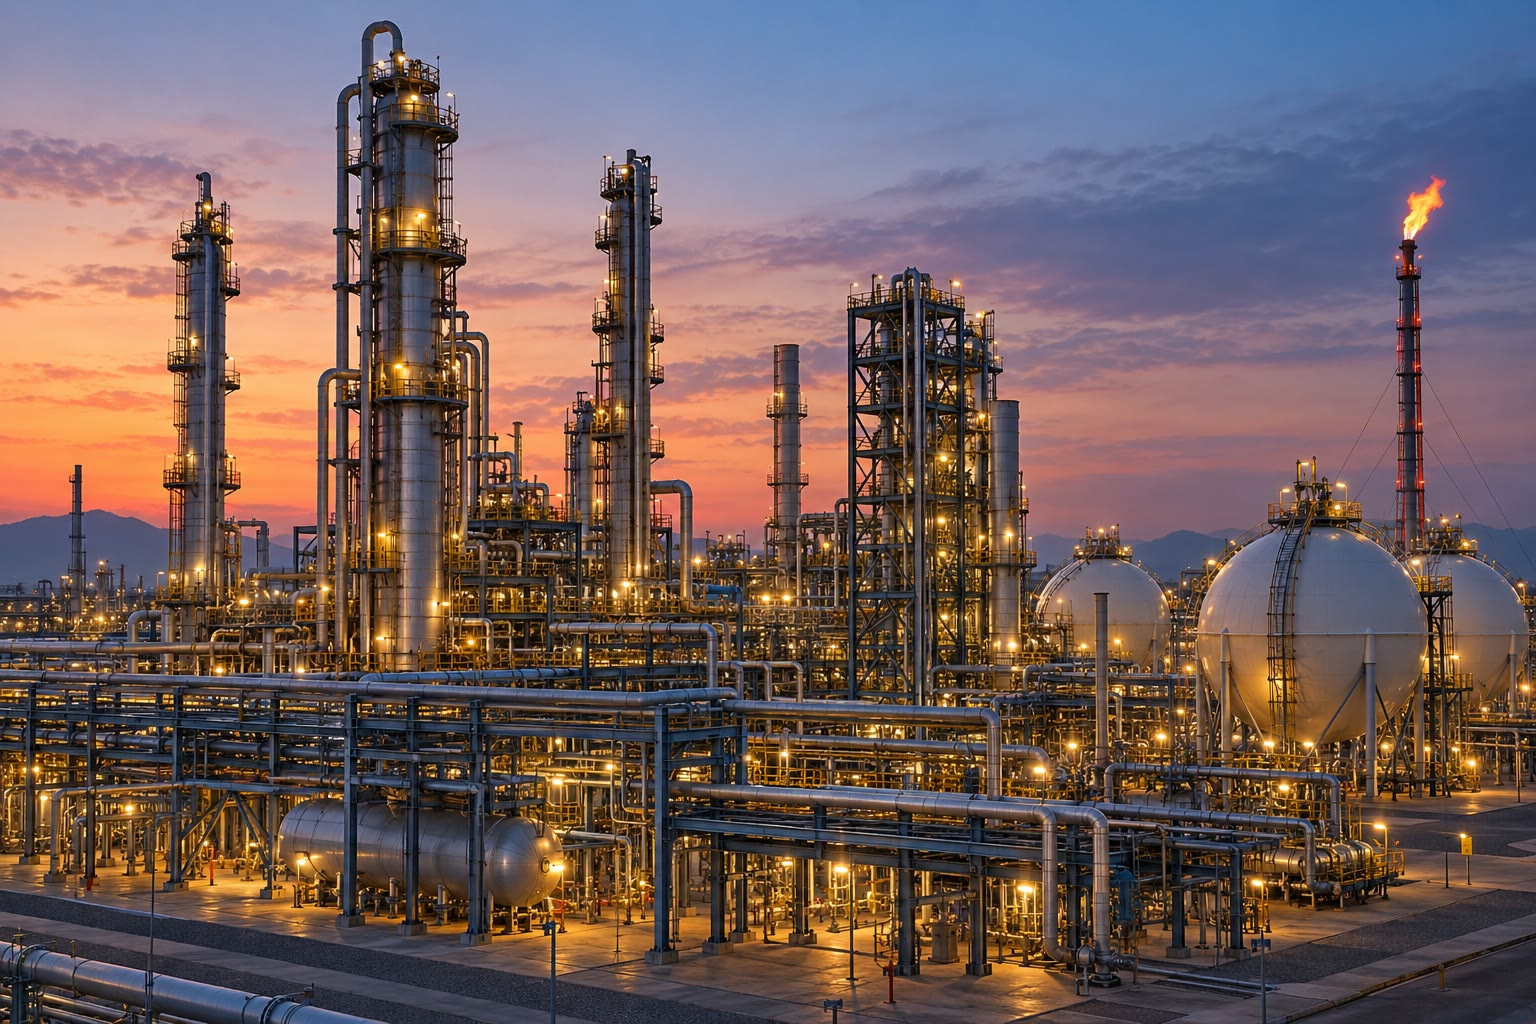
\includegraphics[width=0.6\linewidth]{images/book4/ai/b3-16-ammonia-plant.jpg}

{\small مصنع لتخليق الأمونيا. يحوي المفاعل في قلبه أطنانًا من
حفاز الحديد المعزَّز؛ ومعظم المصنع يحضّر الهيدروجين ويعيد تدوير
الغاز غير المحوَّل.}
\end{omfigure}

\section{فحص السطوح}

\begin{definition}[مطيافية الانتزاز الحراري]\label{def:b3:surfaces-catalysis:tpd}
\emph{مطيافية الانتزاز الحراري}\index{مطيافية الانتزاز الحراري}
تسخّن سطحًا يحمل \omterm{def:b3:surfaces-catalysis:adsorption}{مادة ممتزة} بسرعة ثابتة وتسجّل
الغاز المنتزّ بمطياف كتلة؛ فكل حالة ارتباط تعطي قمة، تزداد
درجة حرارتها مع طاقة تنشيط انتزازها.
\end{definition}

يعطي موضع قمة \omterm{def:b3:surfaces-catalysis:adsorption}{الانتزاز} طاقةَ \omterm{def:b3:surfaces-catalysis:adsorption}{الانتزاز} (من أجل \omterm{def:b3:surfaces-catalysis:adsorption}{انتزاز} من الرتبة
الأولى، $E_d \approx RT_{\mathrm p}[\ln(\nu T_{\mathrm p}/\beta) - 3.64]$ مع $\beta$ سرعة التسخين و$\nu \approx \qty{e13}{s^{-1}}$،
وهو ما نقبله)، وتعطي مساحتها الكمية الممتزة. وتقيس المطيافية الضوئية الإلكترونية بالأشعة
السينية (XPS) طاقات ارتباط الإلكترونات الداخلية لذرات السطح،
التي تعرّف العناصر وحالات أكسدتها في النانومترات القليلة
الأولى. ويحرّك المجهر النفقي الماسح رأسًا حادًا على بعد بضعة أعشار
النانومتر فوق سطح موصل؛ وتيار \omterm{def:b3:quantum-model-systems:tunnelling}{العبور النفقي}
(\cref{ch:b3:quantum-model-systems}) ينخفض بنحو رتبة عشرية لكل
\qty{0.1}{nm} من المسافة الإضافية، بحيث إن إبقاءه ثابتًا في أثناء المسح
يرسم خريطة السطح ذرة ذرة.

\begin{inthelab}[قياس BET]
يوزن نحو \qty{0.2}{g} من العيّنة في أنبوب زجاجي ذي انتفاخ، وتُنزع غازاته
ساعات تحت الفراغ عند 150 إلى \qty{300}{\celsius}، ثم يوزن من جديد، ويُركّب على
الجهاز، والانتفاخ مغمور في وعاء ديوار من النيتروجين السائل. ويُدخل الجهاز
النيتروجين بجرعات صغيرة ويقيس ضغط التوازن بعد كل جرعة،
مستنتجًا الكمية الممتزة من حصيلة الغاز؛ ويُقاس الحجم الميت للأنبوب
بالهيليوم، الذي لا يُمتز.
\end{inthelab}

\begin{safety}{\ghs[0.7cm]{GHS06}\ghs[0.7cm]{GHS07}\ghs[0.7cm]{GHS08}\ghs[0.7cm]{GHS09}}
% ledger: ghs4:V2O5, ghs4:Ni
الحفازات الفلزية المختزلة (النيكل أو البلاديوم أو البلاتين المجزأ تجزئة دقيقة على
حامل، والمختزل حديثًا في الهيدروجين) قد تشتعل عند ملامسة الهواء: فهي
تُتداول تحت غاز خامل وتُخمَّل قبل التخزين. والنيكل يسبب
تحسس الجلد ويُشتبه في أنه مسرطن؛ وأكسيد الفاناديوم(V) سام إذا استُنشق
وإذا ابتُلع وقد يسبب السرطان. وتوزن مساحيق الحفازات في
حيّز مهوّى.
\end{safety}

\begin{history}[لانغموير وحفاز الأمونيا]
اشتق إرفينغ لانغموير، الذي كان يعمل على المصابيح الكهربائية في مختبر صناعي،
متساوي الحرارة الذي يحمل اسمه في 1916--1918 من فكرة أن الغازات الممتزة تكوّن طبقة سمكها
جزيء واحد، ونال جائزة نوبل في الكيمياء لسنة 1932 عن كيمياء
السطوح. وقبل ذلك ببضع سنوات، كان ألفين ميتاش قد نظّم البحث عن
حفاز عملي للأمونيا: فاختُبرت آلاف التراكيب في مفاعلات صغيرة
عالية الضغط قبل أن يُختار حفاز الحديد المعزَّز، الذي لا يزال مستعملًا.
وكان ذلك من أوائل عمليات الغربلة المنهجية للحفازات.
\end{history}

\section{تمارين}

\begin{exercise}[$\star$]\label{exo:b3:surfaces-catalysis:1}
يغطي غاز 40\,\% من سطح لانغموير عند \qty{2.0}{kPa}. احسب $K$ والتغطية عند
\qty{10}{kPa}.
\end{exercise}

\begin{exercise}[$\star$]\label{exo:b3:surfaces-catalysis:2}
قيست أنتالبيا \omterm{def:b3:surfaces-catalysis:adsorption}{امتزاز} على فلز: $-20$ و\qty{-150}{kJ/mol}. أيهما
\omterm{def:b3:surfaces-catalysis:physi-chemi}{امتزاز فيزيائي}، وأيهما \omterm{def:b3:surfaces-catalysis:physi-chemi}{امتزاز كيميائي}؟ وأيهما يمكن أن يكون تفككيًا؟
\end{exercise}

\begin{exercise}[$\star$]\label{exo:b3:surfaces-catalysis:3}
عُدّ، لكل ذرة سطحية، المواقع العلوية والجسرية والتجاويف على وجه (100) 
وعلى وجه (111) لفلز مكعب ممركز الأوجه.
\end{exercise}

\begin{exercise}[$\star$]\label{exo:b3:surfaces-catalysis:4}
يحوّل حفاز \qty{3.0e-6}{mol} من المتفاعل لكل غرام في الثانية ويحمل
\qty{1.5e-5}{mol} من المواقع السطحية لكل غرام. احسب تردد الدوران.
\end{exercise}

\begin{exercise}[$\star\star$]\label{exo:b3:surfaces-catalysis:5}
يُمتز الهيدروجين امتزازًا تفككيًا مع $\theta = 0.10$ عند \qty{1.0}{kPa}. احسب $\theta$ عند \qty{4.0}{kPa}.
\end{exercise}

\begin{exercise}[$\star\star$]\label{exo:b3:surfaces-catalysis:6}
يتنافس CO ($K = \qty{10}{kPa^{-1}}$) و\ce{O2} ($K = \qty{0.5}{kPa^{-1}}$، غير تفككي في هذا النموذج البسيط)
على مواقع سطح من البلاتين عند 1.0 و\qty{5.0}{kPa}. احسب
التغطيتين وعلّق على سرعة أكسدة CO.
\end{exercise}

\begin{exercise}[$\star\star$]\label{exo:b3:surfaces-catalysis:7}
تغطية تُبلغ عند \qty{1.0}{kPa} عند \qty{300}{K} تحتاج إلى \qty{8.0}{kPa} عند \qty{350}{K}. احسب \omterm{def:b3:surfaces-catalysis:isosteric}{أنتالبي
الامتزاز متساوية التغطية}.
\end{exercise}

\begin{exercise}[$\star\star$]\label{exo:b3:surfaces-catalysis:8}
% ledger: sa:N2.am, const:Vm1, const:NA
لكربون منشَّط $v_{\mathrm m} = \qty{120}{cm^3.g^{-1}}$ (الشروط القياسية، 273.15 K 
و\qty{101.325}{kPa}). احسب مساحته وفق BET.
\end{exercise}

\begin{exercise}[$\star\star$]\label{exo:b3:surfaces-catalysis:9}
سرعة التفاعل $\ce{2 CO + O2 -> 2 CO2}$ على البلاتين ترتفع، وتمر بقيمة عظمى ثم تنخفض كلما
ازداد $p(\ce{CO})$ عند $p(\ce{O2})$ ثابت. على أي آلية يدل ذلك، ولماذا يثبّط CO
التفاعل؟
\end{exercise}

\begin{exercise}[$\star\star\star$]\label{exo:b3:surfaces-catalysis:10}
لتفاعل سطحي طاقة تنشيط حقيقية قدرها \qty{100}{kJ/mol}؛ وللمتفاعل
$\Delta_{\mathrm{ads}}H = \qty{-60}{kJ/mol}$. ما طاقة التنشيط المقيسة عند تغطية ضعيفة وعند تغطية
مرتفعة؟ ارسم بخطوط عامة $\ln r$ بدلالة $1/T$ على مجال واسع.
\end{exercise}

\begin{exercise}[$\star\star\star$]\label{exo:b3:surfaces-catalysis:11}
يُمتز الكبريت على حفاز من النيكل بتغطية قدرها 0.10 (ذرات كبريت لكل
ذرة Ni سطحية)، وتسد كل ذرة كبريت أربعة مواقع. ما نسبة النشاط
الباقية لتفاعل يحتاج إلى موقع حر واحد؟ ولتفاعل يحتاج إلى موقعين حرين متجاورين (افترض
أن المواقع المسدودة موزعة عشوائيًا)؟
\end{exercise}

\begin{exercise}[$\star\star\star$]\label{exo:b3:surfaces-catalysis:12}
في تخليق الأمونيا، تربط ثلاثة فلزات النيتروجين الذري بأنتالبيات قدرها
$-150$ و$-250$ و\qty{-400}{kJ/mol} (معطيات التمرين). باستعمال \omterm{def:b3:surfaces-catalysis:sabatier}{مبدأ
ساباتييه}، أيها يُرجَّح أن يكون أفضل حفاز، وما الذي يحدّ الفلزين الآخرين؟
\end{exercise}

\section{مسألة: قياس حفاز}

\begin{problem}[{مسألة نهاية الأسبوع --- قياس حفاز: مساحة BET
لحفاز بلاتين محمول، وتشتت الفلز فيه وحجم جسيماته من
الامتزاز الكيميائي للهيدروجين، وتردد الدوران في تفاعل هدرجة}]
\label{pb:b3:surfaces-catalysis:1}
% ledger: sa:N2.am, lat:Pt, aw:Pt, const:Vm1, const:NA
يحتوي حفاز على 1.00\,\% كتلةً من البلاتين على الألومينا. معطيات المسألة:
متساوي حرارة النيتروجين عند \qty{77}{K} (الأحجام في الشروط القياسية، 273.15 K 
و\qty{101.325}{kPa}، لكل غرام):
\begin{center}\small
\begin{tabular}{lcccccc}
\hline
$x = p/p^*$ & 0.05 & 0.10 & 0.15 & 0.20 & 0.25 & 0.30 \\
$v$ / \unit{cm^3.g^{-1}} & 41.2 & 46.1 & 51.1 & 54.1 & 58.9 & 62.9 \\ \hline
\end{tabular}
\end{center}
\ce{H2} الممتز كيميائيًا على البلاتين: \qty{0.205}{cm^3} لكل غرام من الحفاز. ويجري تفاعل هدرجة
بسرعة \qty{2.0e-5}{mol} لكل غرام من الحفاز في الثانية. البلاتين: $M = \qty{195.08}{g/mol}$، مكعب ممركز الأوجه،
$a = \qty{392.3}{pm}$؛ والحجم المولي لغاز في الشروط القياسية \qty{22414}{cm^3/mol}؛
$a_{\mathrm m}(\ce{N2}) = \qty{0.162}{nm^2}$.

\medskip\noindent\textbf{الجزء الأول --- مخطط BET.}
\begin{enumerate}
  \item لماذا يُقاس متساوي الحرارة عند \qty{77}{K}؟
  \item لماذا لا تُستعمل إلا الضغوط النسبية بين 0.05 و0.30؟
  \item احسب $x/(v(1 - x))$ لكل نقطة.
  \item لمستقيم المربعات الصغرى ميل قدره \num{0.02205} وتقاطع قدره \num{0.000180} (بوحدة
        \unit{g.cm^{-3}}). استنتج $v_{\mathrm m}$.
  \item استنتج $c$. وماذا تعني قيمة كبيرة للثابت $c$؟
  \item لماذا يُحدَّد التقاطع بدقة رديئة إلى هذا الحد، وهل يؤثر ذلك في $v_{\mathrm m}$؟
\end{enumerate}

\medskip\noindent\textbf{الجزء الثاني --- المساحة.}
\begin{enumerate}[resume]
  \item احسب كمية النيتروجين في \omterm{def:b3:surfaces-catalysis:coverage}{الطبقة الأحادية} لكل غرام.
  \item احسب \omterm{def:b3:surfaces-catalysis:surface-area}{المساحة السطحية النوعية}.
  \item أي جزء من الصلب يوفر كل هذه المساحة تقريبًا؟
  \item لماذا تخفق طريقة BET في الصلبة الدقيقة المسام مثل الزيوليتات؟
\end{enumerate}

\medskip\noindent\textbf{الجزء الثالث --- التشتت وحجم الجسيمات.}
\begin{enumerate}[resume]
  \item احسب كمية ذرات H الممتزة كيميائيًا لكل غرام.
  \item احسب كمية البلاتين لكل غرام.
  \item استنتج التشتت.
  \item احسب الحجم لكل ذرة Pt في الكتلة.
  \item المساحة لكل ذرة سطحية، بالمتوسط على الأوجه (111) و(100) و(110)،
        هي \qty{0.0807}{nm^2}. تحقّق من قيمة الوجه (111)، $\frac{\sqrt3}{4}a^2$.
  \item بيّن أنه من أجل الكرات $d = 6v_{\mathrm{at}}/(a_{\mathrm{at}}D)$.
  \item احسب متوسط قطر الجسيمات.
  \item ما الافتراضات التي تحدّ هذه النتيجة؟
\end{enumerate}

\medskip\noindent\textbf{الجزء الرابع --- النشاط.}
\begin{enumerate}[resume]
  \item احسب تردد الدوران لكل ذرة Pt سطحية.
  \item احسب السرعة لكل غرام من البلاتين.
  \item لو تلبّدت الجسيمات حتى \qty{10}{nm} مع بقاء تردد الدوران ثابتًا، فبأي
        عامل تنخفض السرعة لكل غرام؟
  \item ماذا يكشف تردد دوران يتغير مع حجم الجسيمات؟
  \item لماذا تُقارن الحفازات بتردد الدوران بدل السرعة لكل
        غرام؟
  \item اذكر النتيجة: متوسط قطر جسيمات البلاتين.
\end{enumerate}
\end{problem}
